\chapter{A bivariate beta distribution}
\label{appendix:bivariate-beta-distribution}

\textcite{olkin2015constructions} describe a bivariate distribution with beta
marginal distributions, positive probability over the space $[0,1] \times
[0,1]$, and correlations over the full range $(-1,1)$. In this section, we
derive it and analyse some of its consequences as prior distribution. 

\section{Construction of the distribution}

Let $U = (U_1, U_2, U_3, U_4) \sim
\operatorname{Dirichlet}(\boldsymbol{\alpha})$, where $\boldsymbol{\alpha} =
(\alpha_1, \alpha_2, \alpha_3, \alpha_4)$ with $\alpha_i > 0, i = 1,\dots,4$
and $U_4 = 1 - U_1 + U_2 + U_3$. The joint density of $U$ with respect to the
Lebesgue measure is given by
\begin{equation}
  f_U(u_1, u_2, u_3) = \frac{1}{B(\boldsymbol{\alpha})}u_1^{\alpha_1-1}u_2^{\alpha_2-1}u_3^{\alpha_3-1}(1-u_1-u_2-u_3)^{\alpha_4-1}, 
\end{equation}
when $u_i \in [0,1], i = 1,2,3$, $u_1 + u_2 + u_3 \le 1$, and $0$ otherwise.
The normalizing constant is defined for $v \in \R^n$ as
$$B(v) = \frac{\prod_{i=1}^n \Gamma(v_i)}{\Gamma\left(\sum_{i=1}^n v_i\right)}.$$ 
\begin{definition}
  Let 
  \begin{equation}
    X = U_1 + U_2 \text{ and } Y = U_1 + U_3.
  \end{equation} 
    The distribution of $(X,Y)$ is {\em bivariate beta} with parameter
    $\boldsymbol{\alpha}$. 
\end{definition}

\autoref{fig:beta-bivariate} presents the joint density of $X$ and $Y$ for
different values of $\boldsymbol{\alpha}$. The following two propositions describe the marginal and joint
densities of
bivariate beta distribution. Their proofs are in the Appendix. 

\begin{figure}[!ht]
  \centering
  \caption{Joint density of the variables $X$ and $Y$ for different choices of $\boldsymbol{\alpha}$.}
  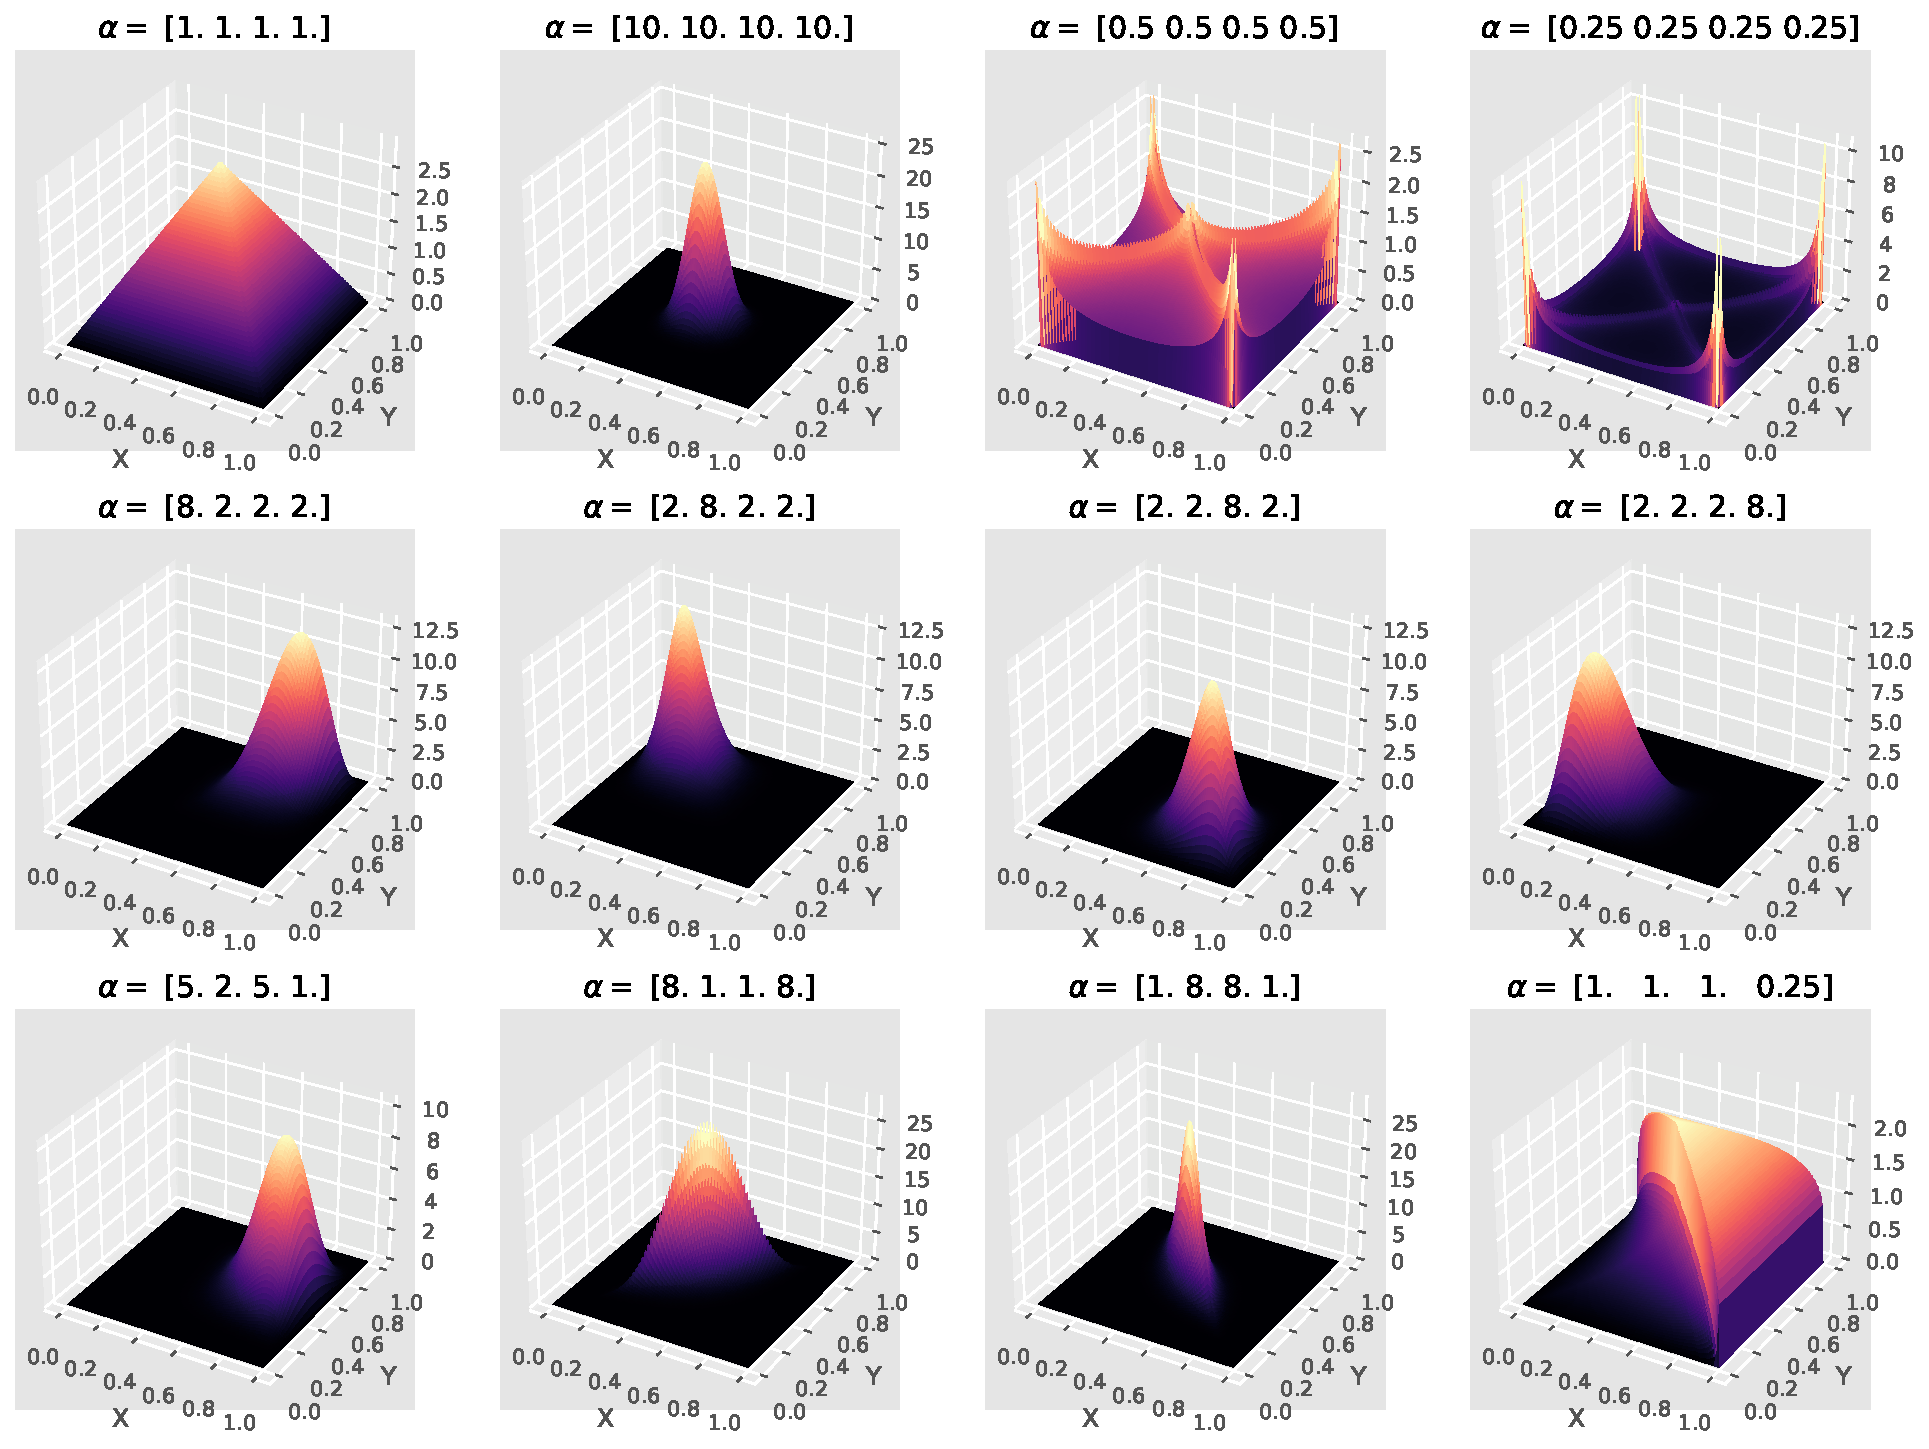
\includegraphics[width=14cm]{joint-densities-bivariate-beta.pdf}
  \fonte{Prepared by the author (2021).}
  \label{fig:beta-bivariate}
\end{figure}

\begin{proposition}[Marginal distributions]
  \label{prop:marginal-distributions}
  The marginal distribution of $X$ is Beta with parameters $\alpha_1 +
  \alpha_2$ and $\alpha_3 + \alpha_4$. Similarly, the marginal distribution of
  $Y$ is Beta with parameters $\alpha_1 + \alpha_3$ and $\alpha_2 + \alpha_4$.
\end{proposition}

\begin{proof}
  First we derive the probability density of $(U_1, U_2)$.
  \begin{equation}
    \label{eq:dist-u1-u2}
    \begin{split}
      f_{U_1, U_2}(u_1, u_2) &= \int_{-\infty}^{\infty} f_{U}(u_1,u_2,u_3) \, du_3 \\ 
      &= \frac{1}{B(\boldsymbol{\alpha})}\int_0^1 u_1^{\alpha_1-1}u_2^{\alpha_2-1}u_3^{\alpha_3-1}(1-u_1-u_2-u_3)^{\alpha_4-1} \, du_3 \\
      &= \frac{1}{B(\boldsymbol{\alpha})}u_1^{\alpha_1-1}u_2^{\alpha_2-1}\int_0^1 u_3^{\alpha_3-1}(1-u_1-u_2-u_3)^{\alpha_4-1} \, du_3.
    \end{split}
  \end{equation}
  Let $u_3 = (1 - u_1 - u_2)z$. Then,
  \begin{equation}
    \begin{split}
      f_{U_1, U_2}(u_1, u_2) &= \frac{1}{B(\boldsymbol{\alpha})}u_1^{\alpha_1-1}u_2^{\alpha_2-1} \\
      &\hspace{1cm} \times \int_0^1 (1-u_1-u_2)^{\alpha_3-1}z^{\alpha_3-1}(1-u_1-u_2)^{\alpha_4}(1-z)^{\alpha_4-1} \, dz. \\
      &= \frac{1}{B(\boldsymbol{\alpha})}u_1^{\alpha_1-1}u_2^{\alpha_2-1}(1-u_1-u_2)^{\alpha_3+\alpha_4-1}\int_0^1 z^{\alpha_3-1}(1-z)^{\alpha_4-1} \, dz. \\
      &= \frac{1}{B(\boldsymbol{\alpha})}u_1^{\alpha_1-1}u_2^{\alpha_2-1}(1-u_1-u_2)^{\alpha_3+\alpha_4-1}\frac{\Gamma(\alpha_3)\Gamma(\alpha_4)}{\Gamma(\alpha_3 + \alpha_4)} \\
      &= \frac{1}{B(\alpha_1, \alpha_2, \alpha_3+\alpha_4)}u_1^{\alpha_1-1}u_2^{\alpha_2-1}(1-u_1-u_2)^{\alpha_3+\alpha_4-1}.
    \end{split}
  \end{equation}

We conclude that
$$(U_1, U_2, 1-U_1-U_2) \sim
\operatorname{Dirichlet}(\alpha_1,\alpha_2,\alpha_3+\alpha_4).$$

Define 
$$
H(v) = \begin{bmatrix}
  1 & 0 \\ 1 & 1
\end{bmatrix}v, \text{ for } v \in \R^2.
$$

Then $(U_1, X) = H(U_1, U_2)$ and $H(\cdot)$ is bijective and differentiable function. By the Change of Variable Formula, 
\begin{equation}
  \begin{split}
    f_{U_1, X}(u_1, x) &= f({H^{-1}(u_1,x)})\bigg|\det\left[\frac{dH^{-1}(v)}{dv}\bigg|_{v=(u_1,x)}\right]\bigg| \\ 
    &= f(u_1, x - u_1) = \frac{1}{B(\alpha_1, \alpha_2, \alpha_3+\alpha_4)}u_1^{\alpha_1-1}(x-u_1)^{\alpha_2-1}(1-x)^{\alpha_3+\alpha_4-1}, 
  \end{split}
\end{equation}
where $(u_1, x)$ belongs to the triangle defined by the points (0,0),
(0,1), and (1,1). The distribution of $X$ for $x \in [0,1]$ is
\begin{equation}
  \begin{split}
    f_X(x) &= \frac{1}{B(\alpha_1, \alpha_2, \alpha_3+\alpha_4)}\int_{0}^{x} u_1^{\alpha_1-1}(x-u_1)^{\alpha_2-1}(1-x)^{\alpha_3+\alpha_4-1} \, du_1 \\
    &= \frac{1}{B(\alpha_1, \alpha_2, \alpha_3+\alpha_4)}(1-x)^{\alpha_3+\alpha_4-1} \int_{0}^{x} u_1^{\alpha_1-1}(x-u_1)^{\alpha_2-1} \, du_1. \\
    &= \frac{1}{B(\alpha_1, \alpha_2, \alpha_3+\alpha_4)}(1-x)^{\alpha_3+\alpha_4-1} \\
    &\hspace{1cm}\times \int_{0}^{x} x^{\alpha_1-1} \left(\frac{u_1}{x}\right)^{\alpha_1-1}x^{\alpha_2 - 1}\left(1-\frac{u_1}{x}\right)^{\alpha_2-1} \, du_1. \\
  \end{split}
\end{equation}

Setting $u = u_1/x$ (if $x = 0, f_X(x) = 0$, then suppose $x > 0$), we have, 
\begin{equation}
  \begin{split}
    f_X(x) &= \frac{1}{B(\alpha_1, \alpha_2, \alpha_3+\alpha_4)}(1-x)^{\alpha_3+\alpha_4-1} x^{\alpha_1+\alpha_2-1} \int_{0}^{1} u^{\alpha_1-1}(1-u)^{\alpha_2-1} \, du. \\
    &= \frac{1}{B(\alpha_1, \alpha_2, \alpha_3+\alpha_4)}(1-x)^{\alpha_3+\alpha_4-1} x^{\alpha_1+\alpha_2-1} B(\alpha_1, \alpha_2)\\
    &= \frac{1}{B(\alpha_1 + \alpha_2, \alpha_3+\alpha_4)}(1-x)^{\alpha_3+\alpha_4-1} x^{\alpha_1+\alpha_2-1}\\
  \end{split}
\end{equation}
Therefore $X \sim \betadist(\alpha_1+\alpha_2, \alpha_3+\alpha_4)$. Similarly $Y \sim \betadist(\alpha_1+\alpha_3, \alpha_2 + \alpha_4)$.
\end{proof}

From the marginal distributions, we already know the expected values and variances of the random variables $X$ and $Y$. Denote $\tilde{\alpha} = \sum_{i=1}^4 \alpha_i$ and we have 

\begin{gather}
    \begin{aligned}
    \ev[X] &= \frac{\alpha_1 + \alpha_2}{\tilde{\alpha}},
    & \ev[Y] &= \frac{\alpha_1 + \alpha_3}{\tilde{\alpha}},
    \\
    \var[X] &= \frac{(\alpha_1 + \alpha_2)(\alpha_3 + \alpha_4)}{\tilde{\alpha}^2(\tilde{\alpha} + 1)},
    & \var[Y] &= \frac{(\alpha_1 + \alpha_3)(\alpha_2 + \alpha_4)}{\tilde{\alpha}^2(\tilde{\alpha} + 1)}.
    \end{aligned}
\end{gather}

\begin{proposition}[Bivariate beta density]
  \label{prop:bivariate-beta-density}
  The joint density of $(X,Y)$ with respect to the Lebesgue measure is
  given by 
  \begin{equation}
    f_{X,Y}(x,y) = \frac{1}{B(\boldsymbol{\alpha})}\int_{\Omega} u_1^{\alpha_1 - 1}(x - u_1)^{\alpha_2 -1}(y-u_1)^{\alpha_3-1}(1-x-y+u_1)^{\alpha_4-1} \, du_1,
  \end{equation}
  where 
  $$
  \Omega = (\max(0, x+y-1), \min(x,y)).
  $$
\end{proposition}

\begin{proof}
  Note that
  $$
  \begin{bmatrix}
    U_1 \\ X \\ Y
  \end{bmatrix}  = \begin{bmatrix}
    1 & 0 & 0 \\
    1 & 1 & 0 \\
    1 & 0 & 1
  \end{bmatrix}\begin{bmatrix}
    U_1 \\ U_2 \\ U_3
  \end{bmatrix}, 
  $$
  where the linear function is bijective and differentiable function, such
  that the determinant of the derivative is 1. By the Change of Variable
  Formula, 
  \begin{equation}
    \begin{split}
      f_{U_1,X,Y}(u_1,x,y) &= f_{U_1,U_2,U_3}(u_1, x - u_1, y - u_2) \\ 
      &= \frac{1}{B(\boldsymbol{\alpha})}u_1^{\alpha_1-1}(x-u_1)^{\alpha_2-1}(y-u_1 )^{\alpha_3-1}(1-x-y+u_1)^{\alpha_4-1},
    \end{split}
  \end{equation}
  where $0 \le u_1 \le x, u_1 \le y$, and $0 \le 1 - x - y + u_1$.  
  Hence,
  \begin{equation}
      \label{eq:dist-X-Y}
      f_{X,Y}(x,y) = \frac{1}{B(\boldsymbol{\alpha})}\int_{\Omega} u_1^{\alpha_1-1}(x-u_1)^{\alpha_2-1}(y-u_1)^{\alpha_3-1}(1-x-y+u_1)^{\alpha_4-1} \, du_1,
  \end{equation}
  such that $\Omega = \{u_1 : \max(0, x + y -1) < u_1 < \min(x,y)\}$.
\end{proof}

At last we derive the covariance and the correlation between $X$ and $Y$.

\begin{proposition}[Covariance and correlation]
  The covariance between $X$ and $Y$ is 
  $$\cov(X,Y) = \frac{1}{\tilde{\alpha}^2(\tilde{\alpha}+1)}(\alpha_1\alpha_4 - \alpha_2\alpha_3)$$
  and
  $$\cor(X,Y) = \frac{\alpha_1\alpha_4 - \alpha_2\alpha_3}{\sqrt{(\alpha_1+\alpha_2)(\alpha_3+\alpha_4)(\alpha_1+\alpha_3)(\alpha_2+\alpha_4)}}$$
\end{proposition}

\begin{proof}

  The covariance between $U_i$ and $U_j$ is \cite[p. 11]{lin2016dirichlet} 
\begin{equation}
  \cov(U_i, U_j) = - \frac{\alpha_i\alpha_j}{\tilde{\alpha}^2(\tilde{\alpha}+1)}, i,j = 1,...,4, i \neq j
\end{equation} 
and the variance of $U_i$ is 
\begin{equation}
  \var(U_i) = \frac{\alpha_i(\tilde{\alpha}-\alpha_i)}{\tilde{\alpha}^2(\tilde{\alpha}+1)},
\end{equation}
since $U_i \sim \operatorname{Beta}(\alpha_i, \tilde{\alpha} -\alpha_i)$.
Therefore 
\begin{equation}
  \cov(X,Y) = \cov(U_1+U_2, U_1+U_3) = \frac{1}{\tilde{\alpha}^2(\tilde{\alpha}+1)}(\alpha_1\alpha_4 - \alpha_2\alpha_3)
\end{equation}
  
\end{proof}

\section{Comments about integration}

The density of $(X,Y)$ is $f_{X,Y}(x,y)$ as in equation \eqref{eq:dist-X-Y}. Therefore it can be undefined in sets of null Lebesgue measure in $\R^2$ and these sets may be important when plotting in a grid, for instance. This section illustrates one of these sets. If $\alpha_i \ge 1,
\, i = 1,...,4$, the integral is clearly well defined for every $x,y \in [0,1]$. Let $0 < \alpha_2 = \alpha_3 = a \le 0.5$ and $x = y < 0.5$. Then
\begin{equation*}
  \begin{split}
    f_{X,Y}(x,y) &= \frac{1}{B(\boldsymbol{\alpha})}\int_{0}^x u_1^{\alpha_1-1}(x-u_1)^{a-1}(x-u_1)^{a-1}(1-2x+u_1)^{\alpha_4-1} \, du_1 \\
    &= \frac{1}{B(\boldsymbol{\alpha})}\int_{0}^{x/2} u_1^{\alpha_1-1}(x-u_1)^{2a-2}(1-2x+u_1)^{\alpha_4-1} \, du_1 + \\
    &~~~+ \frac{1}{B(\boldsymbol{\alpha})}\int_{x/2}^x u_1^{\alpha_1-1}(x-u_1)^{2a-2}(1-2x+u_1)^{\alpha_4-1} \, du_1
  \end{split}
\end{equation*}

Note that the first integral is well defined and non-negative. On the other hand, the second integral is not defined: 
\begin{equation*}
  \begin{split}
    \int_{x/2}^{x} u_1^{\alpha_1-1}&(x-u_1)^{2a-2}(1-2x+u_1)^{\alpha_4-1} \, du_1 \\
    &\ge \int_{x/2}^x \min\left(\left(\frac{x}{2}\right)^{\alpha_1-1}, x^{\alpha_1-1}\right)(x-u_1)^{2a-2} \\ 
    &\hspace{3cm} \times \min\left(\left(1-\frac{3}{2}x\right)^{\alpha_4-1}, (1-x)^{\alpha_4-1}\right) \, du_1 \\
    &= K(x) \int_{0}^{x/2} v^{2a-2} \, dv \\ 
    &= \begin{cases}
      \dfrac{K(x)}{2a-1} \lim_{t \to 0^+} \left[(x/2)^{2a-1} - t^{2a-1}\right] &\text{ if } a < 0.5 \\ 
      K(x) \lim_{t \to 0^+} \left[\log(x/2) - \log(t)\right] &\text{ if } a = 0.5
    \end{cases} \\
    &\to +\infty, 
  \end{split}
\end{equation*}
where $K(x)$ is a function of $x$. 

Based on this divergence, we conclude that if $0 < \alpha_2 = \alpha_3 \le 0.5$
and $x = y < 0.5$, $f_{X,Y}(x,y)$ is not defined. Notice that if $x = y \ge
0.5$, divergence problems still happens, since the problems appear when $u_1$ approximates $x$. Similar calculations show that if $x + y = 1$ and $0 < \alpha_1 = \alpha_4 \le 0.5$, the density is also
not defined. More generally, $f_{X,Y}(x,y)$ is not defined if $\alpha_1 +
\alpha_4 \le 1$ and $x + y = 1$; $\alpha_2 + \alpha_3 \le 1$ and $x = y$.

\section{Elicitation of a bivariate beta}

Suppose that it is known the following moments of the Bivariate Beta distribution: $m_1 = \ev[X], m_2 = \ev[Y], v_1 = \var(X), v_2 = \var(Y)$, and $\rho  = \cor(X,Y)$. Notice that $v_1 + m_1^2 = \var(X_1) + \ev[X_1]^2 = \ev[X_1^2]$ and
$$
\ev[X_1^2] - \ev[X_1] = \frac{(\alpha_1 + \alpha_2 + 1)(\alpha_1 + \alpha_2)}{(\tilde{\alpha} + 1)\tilde{\alpha}} - \frac{\alpha_1 + \alpha_2}{\tilde{\alpha}} = -\frac{(\alpha_1 + \alpha_2)(\alpha_3 + \alpha_4)}{\tilde{\alpha}(\tilde{\alpha}+1)} < 0, 
$$
that is, $v_1 + m_1^2 - m_1 < 0 \implies v_1 < m_1 - m_1^2$ and similarly,
$v_2 < m_2 - m_2^2$. After fixing these quantities, we will have a non-linear system with five equations and four
unknown variables. Hence, we want to solve the following 
\begin{equation}
  \label{eq:system-moments-alpha}
  \begin{cases}
    m_1 = \dfrac{\alpha_1+\alpha_2}{\tilde{\alpha}} \\
    m_2 = \dfrac{\alpha_1+\alpha_3}{\tilde{\alpha}} \\ 
    v_1 = \dfrac{(\alpha_1+\alpha_2)(\alpha_3+\alpha_4)}{\tilde{\alpha}^2(\tilde{\alpha}+1)} \\
    v_2 = \dfrac{(\alpha_1+\alpha_3)(\alpha_2+\alpha_4)}{\tilde{\alpha}^2(\tilde{\alpha}+1)} \\
    \rho = \dfrac{\alpha_1\alpha_4 - \alpha_2\alpha_3}{\sqrt{(\alpha_1+\alpha_2)(\alpha_3+\alpha_4)(\alpha_1+\alpha_3)(\alpha_2+\alpha_4)}}
  \end{cases}
\end{equation}

Notice that we can simplify the third and fourth equations since 
$$
\frac{\alpha_3 + \alpha_4}{\tilde{\alpha}} = \frac{\tilde{\alpha} - (\alpha_1 + \alpha_2)}{\tilde{\alpha}} = 1 - m_1 
$$
and analogously, 
$$
\frac{\alpha_2 + \alpha_4}{\tilde{\alpha}} = 1 - m_2. 
$$
Therefore, 
\begin{align*}
    v_1 &= \frac{m_1(1 - m_1)}{\tilde{\alpha} + 1} \\
    v_2 &= \frac{m_2(1 - m_2)}{\tilde{\alpha} + 1}
\end{align*}

This already tells us that the system do not have a solution if 
$$
\frac{m_1(1-m_1)}{v_1} \neq \frac{m_2(1-m_2)}{v_2}. 
$$

The following proposition builds a solution excluding the fourth equation, given the above comment. 

\begin{proposition}
  System \eqref{eq:system-moments-alpha} without the fourth equation has a unique solution given by 
\begin{gather}
 \label{eq:system-solution}
 \begin{aligned}
  \alpha_1 &= (m_1 + m_2 - 1)\tilde{\alpha} + \alpha_4 \\
  \alpha_2 &=  (1 - m_2)\tilde{\alpha} - \alpha_4 \\
  \alpha_3 &= (1-m_1)\tilde{\alpha} - \alpha_4. \\
  \alpha_4 &= \rho\tilde{\alpha}\sqrt{m_1m_2(1-m_1)(1-m_2)} + (1-m_1)(1-m_2),
\end{aligned}
\end{gather}
where $\tilde{\alpha}$ is given by the expression 
$$
\tilde{\alpha} = \frac{(m_1 - m_1^2 - v_1)}{v_1}.
$$
\end{proposition}

\begin{proof}
  The first two equations of the system \eqref{eq:system-moments-alpha} can be
rewritten as a linear system:
\begin{align*}
  (m_1 - 1)\alpha_1 + (m_1 - 1)\alpha_2 + m_1\alpha_3 + m_1\alpha_4 &= 0 \\
  (m_2 - 1)\alpha_1 + m_2\alpha_2 + (m_2-1)\alpha_3 + m_2\alpha_4 &= 0,   
\end{align*}
which is equivalent to 
\begin{align*}
  \alpha_1 + \alpha_2 + \frac{m_1}{m_1-1}\alpha_3 + \frac{m_1}{m_1-1}\alpha_4 &= 0 \\
  \alpha_2 + \frac{1-m_2}{m_1-1}\alpha_3 + \frac{m_1-m_2}{m_1-1}\alpha_4 &= 0.
\end{align*}
Then, we can write $\alpha_1$ and $\alpha_2$ as functions of $\alpha_3$ and
$\alpha_4$:
\begin{align}
  \alpha_1 &= \frac{m_1+m_2-1}{1-m_1}\alpha_3 + \frac{m_2}{1-m_1}\alpha_4 \\
  \alpha_2 &= \frac{1-m_2}{1-m_1}\alpha_3 + \frac{m_1-m_2}{1-m_1}\alpha_4.
\end{align}

Based on that expression, denote $\alpha_1 = a_3\alpha_3 + a_4\alpha_4$, $\alpha_2
= b_3\alpha_3 + b_4\alpha_4$, $c_3 = a_3 + b_3 + 1$, and $c_4 = a_4 + b_4 + 1$. Then, the third equation can be written as 
$$
a_3\alpha_3 + a_4\alpha_4 + b_3\alpha_3 + b_4\alpha_4 + \alpha_3 + \alpha_4 + 1 = c_3\alpha_3 + c_4 \alpha_4 = \frac{m_1(1-m_1)}{v_1} - 1, 
$$
which implies that 
$$
\alpha_3 = \frac{m_1(1-m_1) - v_1 - c_4v_1\alpha_4}{c_3v_1},
$$
that is a linear function of $\alpha_4$. We summarize the expressions in function of $\alpha_4$ with some simplifications: 
\begin{align*}
  \alpha_1 &= (m_1 + m_2 - 1)\frac{(m_1 - m_1^2 - v_1)}{v_1} + \alpha_4 \\
  \alpha_2 &=  (1 - m_2)\frac{(m_1 - m_1^2 - v_1)}{v_1} - \alpha_4 \\
  \alpha_3 &= (1-m_1)\frac{(m_1 - m_1^2 - v_1)}{v_1} - \alpha_4, \\
\end{align*}
which implies that 
$$
\tilde{\alpha} = \frac{m_1 - m_1^2 - v_1}{v_1}.
$$

Now rewrite the fifth equation using the first two equations from system \eqref{eq:system-moments-alpha} as follows 
\begin{equation*}
    \label{eq:rho-equation}
    \begin{split}
        \rho &= \frac{\alpha_1\alpha_4 - \alpha_2\alpha_3}{\sqrt{(\alpha_1+\alpha_2)(\alpha_3+\alpha_4)(\alpha_1+\alpha_3)(\alpha_2+\alpha_4)}} \\ 
        &= \frac{\alpha_1\alpha_4 - \alpha_2\alpha_3}{\tilde{\alpha}^2\sqrt{m_1m_2(1-m_1)(1-m_2)}} \\ 
        &= \frac{(m_1 + m_2 - 1)\tilde{\alpha}\alpha_4 + \alpha_4^2 - ((1-m_2)\tilde{\alpha} - \alpha_4)((1-m_1)\tilde{\alpha} - \alpha_4)}{\tilde{\alpha}^2\sqrt{m_1m_2(1-m_1)(1-m_2)}} \\
        &= \frac{\alpha_4 - (1-m_1)(1-m_2)\tilde{\alpha}}{\tilde{\alpha}\sqrt{m_1m_2(1-m_1)(1-m_2)}} \\ 
    \end{split}
\end{equation*}
and the solution is, therefore, 
$$
\alpha_4 = \rho\tilde{\alpha}\sqrt{m_1m_2(1-m_1)(1-m_2)} + (1-m_1)(1-m_2).
$$
\end{proof}

Besides the system \eqref{eq:system-moments-alpha}, the Beta Distribution needs that $\alpha_1, \dots, \alpha_4 > 0$. However, this is not necessarily true. Since it is difficult to find the subset $D \subset [0,1]^4$ in which the solution for \eqref{eq:system-solution} is strictly positive for $\alpha_1, \dots, \alpha_4$, we present some examples in Figure \ref{fig:alpha-solutions}.

% \begin{figure}[!hb]
%     \centering
%     \caption{Verification of positivity of the solution for different and fixed values of $v_1$ and $\rho$, and $m_1, m_2 \in [0,1]^2$. The gray region specifies when $m_1 - m_1^2 \le v_1$, which is not possible for beta distribution.}
%     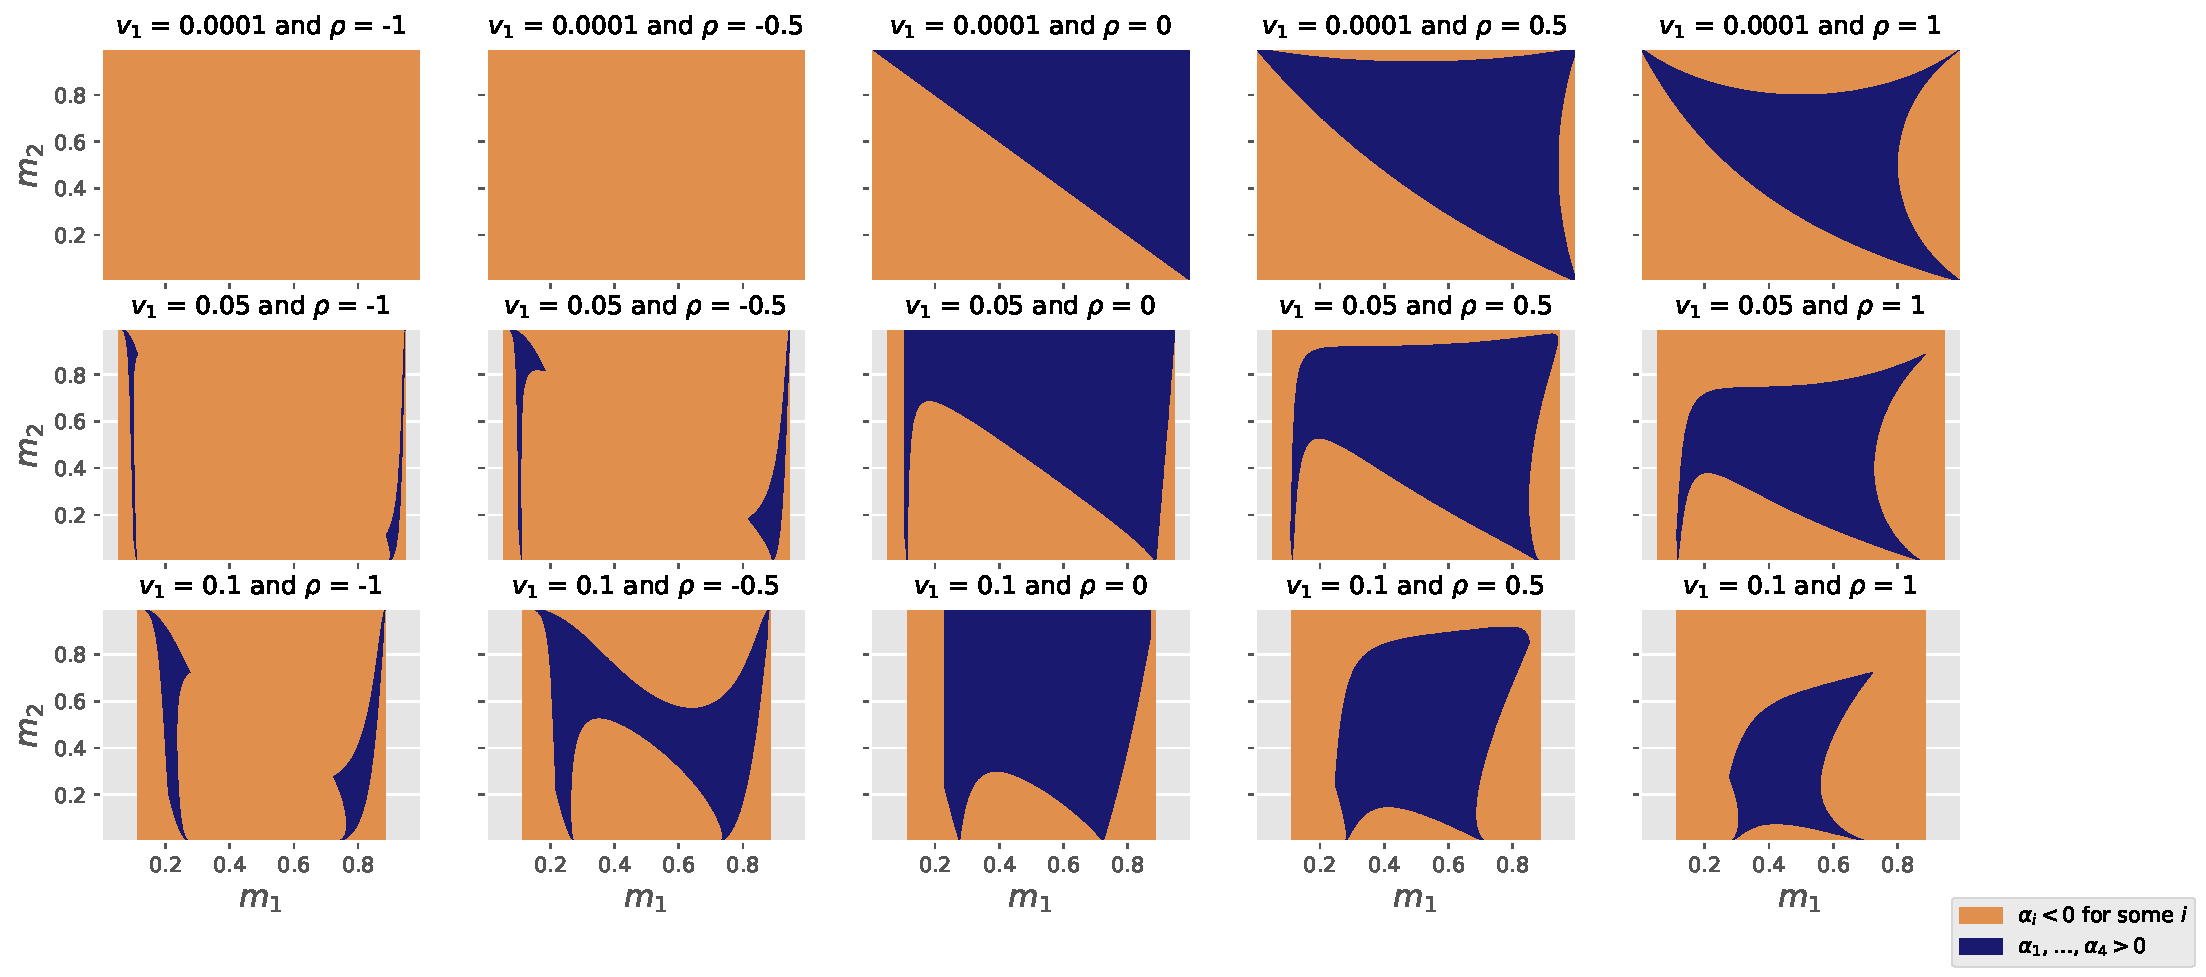
\includegraphics[width=\textwidth]{alpha_solution_existence.eps}
%     \label{fig:alpha-solutions}
% \end{figure}

When $\rho = -1$ for instance, only a few specifications of $m_1$ and $m_2$ generate a solution strictly positive. These examples show that several interesting specifications for the researchers can lead to a non positive solution, as we will see in next section. 


% \section{Specifying parameters
% \texorpdfstring{$\boldsymbol{\alpha}$}{alpha}}

% Suppose that the researcher has knowledge about the main moments of $X$ and
% $Y$, such that $\ev(X) = m_1 \in (0,1), \ev(Y) = m_2 \in (0,1), \var(X) = v_1
% \in (0, 1),$ and $\var(Y) =
% v_2 \in (0,1)$. Notice that $v_1 + m_1^2 = \var(X_1) + \ev[X_1]^2 = \ev[X_1^2]$ and
% $$
% \ev[X_1^2] - \ev[X_1] = \frac{(\alpha_1 + \alpha_2 + 1)(\alpha_1 + \alpha_2)}{(\tilde{\alpha} + 1)\tilde{\alpha}} - \frac{\alpha_1 + \alpha_2}{\tilde{\alpha}} = -\frac{(\alpha_1 + \alpha_2)(\alpha_3 + \alpha_4)}{\tilde{\alpha}(\tilde{\alpha}+1)} < 0, 
% $$
% that is, $v_1 + m_1^2 - m_1 < 0 \implies v_1 < m_1 - m_1^2$ and similarly,
% $v_2 < m_2 - m_2^2$. After fixing these quantities, we will have a non-linear system with four equations and four
% unknown variables. Hence, we want to solve the following 
% \begin{equation}
%   \label{eq:system-moments-alpha}
%   \begin{cases}
%     m_1 = \dfrac{\alpha_1+\alpha_2}{\tilde{\alpha}} \\
%     m_2 = \dfrac{\alpha_1+\alpha_3}{\tilde{\alpha}} \\ 
%     v_1 = \dfrac{(\alpha_1+\alpha_2)(\alpha_3+\alpha_4)}{\tilde{\alpha}^2(\tilde{\alpha}+1)} = m_1\dfrac{\alpha_3+\alpha_4}{\tilde{\alpha}(\tilde{\alpha}+1)} \\
%     v_2 = \dfrac{(\alpha_1+\alpha_3)(\alpha_2+\alpha_4)}{\tilde{\alpha}^2(\tilde{\alpha}+1)} = m_2\dfrac{\alpha_2+\alpha_4}{\tilde{\alpha}(\tilde{\alpha}+1)}.
%   \end{cases}
% \end{equation}

% \begin{proposition}
%   System \eqref{eq:system-moments-alpha} has a solution if, and only if, the relation
%   \begin{equation}
%     \label{eq:v2}
%     v_2 = \frac{(1 - m_2)\tilde{\alpha}}{\tilde{\alpha}(\tilde{\alpha}+ 1)} = \frac{1 - m_2}{\frac{m_1 - m_1^2}{v_1}} = \frac{v_1(1 - m_2)}{m_1(1-m_1)},
%   \end{equation}
%   is satisfied. When there is a solution, there will be
%   infinitely many and they all lay in the ray 
%   $$
% \mathcal{L} = \{(1,-1,-1,1)\alpha_4 + k : \alpha_4 > 0\}, 
% $$
% such that $k = \left((m_1 + m_2 - 1)\tilde{\alpha}, (1-m_2)\tilde{\alpha},
% (1-m_1)\tilde{\alpha}, 0\right)$. 
% \end{proposition}

% \begin{proof}

% The first two equations of the system \eqref{eq:system-moments-alpha} can be
% rewritten as a linear system:
% \begin{align*}
%   (m_1 - 1)\alpha_1 + (m_1 - 1)\alpha_2 + m_1\alpha_3 + m_1\alpha_4 &= 0 \\
%   (m_2 - 1)\alpha_1 + m_2\alpha_2 + (m_2-1)\alpha_3 + m_2\alpha_4 &= 0,   
% \end{align*}
% which is equivalent to 
% \begin{align*}
%   \alpha_1 + \alpha_2 + \frac{m_1}{m_1-1}\alpha_3 + \frac{m_1}{m_1-1}\alpha_4 &= 0 \\
%   \alpha_2 + \frac{1-m_2}{m_1-1}\alpha_3 + \frac{m_1-m_2}{m_1-1}\alpha_4 &= 0.
% \end{align*}
% Then, we can write $\alpha_1$ and $\alpha_2$ as functions of $\alpha_3$ and
% $\alpha_4$:
% \begin{align}
%   \alpha_1 &= \frac{m_1+m_2-1}{1-m_1}\alpha_3 + \frac{m_2}{1-m_1}\alpha_4 \\
%   \alpha_2 &= \frac{1-m_2}{1-m_1}\alpha_3 + \frac{m_1-m_2}{1-m_1}\alpha_4.
% \end{align}
% With that expression, let $\alpha_1 = a_3\alpha_3 + a_4\alpha_4$ and $\alpha_2
% = b_3\alpha_3 + b_4\alpha_4$. Denote $c_3 = a_3 + b_3 + 1$ and $c_4 = a_4 +
% b_4 + 1$. Then, consider the third equation of the system
% \eqref{eq:system-moments-alpha}, 
% \begin{equation*}
%   \begin{split}
%     &\frac{v_1}{m_1} = \frac{\alpha_3+\alpha_4}{\tilde{\alpha}(\tilde{\alpha} +1)} = \frac{\alpha_3+\alpha_4}{(\alpha_1+\alpha_2+\alpha_3+\alpha_4)^2 + (\alpha_1+\alpha_2+\alpha_3+\alpha_4)} \\
%      &\implies \frac{v_1}{m_1}(\alpha_1 + \alpha_2 + \alpha_3 + \alpha_4)^2 = \alpha_3 + \alpha_4 - \frac{v_1}{m_1}(\alpha_1 + \alpha_2 + \alpha_3 + \alpha_4) \\
%     &\implies \frac{v_1}{m_1}(c_3\alpha_3 + c_4\alpha_4)^2 = \left(1-\frac{v_1}{m_1}c_3\right)\alpha_3 + \left(1-\frac{v_1}{m_1}c_4\right)\alpha_4 \\
%     &\implies \frac{v_1c_3^2}{m_1}\alpha_3^2 + \left(\frac{2v_1c_3c_4\alpha_4+v_1c_3}{m_1} - 1\right)\alpha_3 + \left(\frac{v_1c_4^2\alpha_4^2 + v_1c_4\alpha_4}{m_1} - \alpha_4\right) = 0 \\ 
%     &\implies v_1c_3^2\alpha_3^2 + (2v_1c_3c_4\alpha_4+v_1c_3 - m_1)\alpha_3 + (v_1c_4^2\alpha_4^2 + v_1c_4\alpha_4 - m_1\alpha_4) = 0.
%   \end{split}
% \end{equation*}
% Using a Computer Algebra System (CAS) with the Python library SymPy, the above
% expression can be simplified as follows:
% $$
% v_1\alpha_3^2 + \left(v_1(1-m_1) + 2v_1\alpha_4 - m_1(1-m_1)^2\right)\alpha_3 - \alpha_4m_1(1-m_1)^2 + \alpha_4v_1(1 - m_1) + v_1\alpha_4^2 = 0.
% $$
% This way, the solutions of the above equation are function of $\alpha_4$.
% Therefore, after solving the equations, we can use the last equation of the
% system \eqref{eq:system-moments-alpha} as a function on of $\alpha_4$. Let, 
% $$
% \Lambda = \left(v_1(1-m_1) + v_1\alpha_4 - m_1(1-m_1)^2\right).
% $$
% Then, 
% \begin{equation*}
%   \begin{split}
%     \Delta &= \left(v_1(1-m_1) + 2v_1\alpha_4 - m_1(1-m_1)^2\right)^2 - 4v_1(\alpha_4v_1(1 - m_1) - \alpha_4m_1(1-m_1)^2 + v_1\alpha_4^2), \\
%     &= \left(\Lambda + v_1\alpha_4\right)^2 - 4v_1\alpha_4\Lambda \\
%     &= \Lambda^2 - 2\Lambda v_1\alpha_4 + (v_1\alpha_4)^2 \\
%     &= (\Lambda - v_1\alpha_4)^2 \\
%     &= \left(v_1(1-m_1) - m_1(1-m_1)^2\right)^2 \\ 
%     &= (1 - m_1)^2(v_1 + m_1^2 - m_1)^2.
%   \end{split}
% \end{equation*}
% Note that $v_1 + m_1^2 = \var(X_1) + \ev[X_1]^2 = \ev[X_1^2]$ and
% $$
% \ev[X_1^2] - \ev[X_1] = \frac{(\alpha_1 + \alpha_2 + 1)(\alpha_1 + \alpha_2)}{(\tilde{\alpha} + 1)\tilde{\alpha}} - \frac{\alpha_1 + \alpha_2}{\tilde{\alpha}} = -\frac{(\alpha_1 + \alpha_2)(\alpha_3 + \alpha_4)}{\tilde{\alpha}(\tilde{\alpha}+1)} < 0.
% $$
% Therefore, 
% $$
% \sqrt{\Delta} = (1-m_1)(m_1 - v_1 - m_1^2)
% $$
% and 
% \begin{equation*}
%   \begin{split}
%     \alpha_3 &= \frac{1}{2v_1}\left(\left(m_1(1-m_1)^2 - v_1(1-m_1) - 2v_1\alpha_4\right) \pm (1-m_1)(m_1 - v_1 - m_1^2)\right) \\
%     &= - \alpha_4 + \frac{(1-m_1)(m_1 - m_1^2 - v_1) \pm (1-m_1)(m_1-v_1-m_1^2)}{2v_1}.
%   \end{split}
% \end{equation*}
% When the sign is negative, we have that $\alpha_3 = - \alpha_4$, an impossible
% solution. Then, 
% $$
% \alpha_3 = \frac{(1-m_1)(m_1 - m_1^2 - v_1)}{v_1} - \alpha_4.
% $$

% We summarize the expressions in function of $\alpha_4$: 
% \begin{align*}
%   \alpha_3 &= \frac{(1-m_1)(m_1 - m_1^2 - v_1)}{v_1} - \alpha_4 \\
%   \alpha_1 &= \frac{m_1+m_2-1}{1-m_1}\alpha_3 + \frac{m_2}{1-m_1}\alpha_4 = \frac{(m_1 + m_2 - 1)(m_1 - m_1^2 - v_1)}{v_1} + \alpha_4 \\
%   \alpha_2 &= \frac{1-m_2}{1-m_1}\alpha_3 + \frac{m_1-m_2}{1-m_1}\alpha_4 = \frac{(1 - m_2)(m_1 - m_1^2 - v_1)}{v_1} - \alpha_4 .
% \end{align*}

% From here, one can calculate that
% $$
% \tilde{\alpha} = \frac{m_1 - m_1^2 - v_1}{v_1}.
% $$
% Since $\alpha_2 + \alpha_4 = (1 - m_2)\tilde{\alpha}$, we have that the last
% equation of the system \eqref{eq:system-moments-alpha} is given by
% \eqref{eq:v2}, that is, the system $\eqref{eq:system-moments-alpha}$ has a solution if and
% only if, equation \eqref{eq:v2} is satisfied. If it is, the solution is the ray 
% $$
% \mathcal{L} = \{(1,-1,-1,1)\alpha_4 + k : \alpha_4 > 0\}, 
% $$
% such that $k = \left((m_1 + m_2 - 1)\tilde{\alpha}, (1-m_2)\tilde{\alpha},
% (1-m_1)\tilde{\alpha}, 0\right)$. 

% \end{proof}


% Now change the fourth equation of \eqref{eq:system-moments-alpha} by: 
% $$
% \cor(X,Y) = \frac{\alpha_1\alpha_4 - \alpha_2\alpha_3}{\sqrt{(\alpha_1+\alpha_2)(\alpha_3+\alpha_4)(\alpha_1+\alpha_3)(\alpha_2+\alpha_4)}} = \frac{\alpha_1\alpha_4 - \alpha_2\alpha_3}{\tilde{\alpha}^2\sqrt{m_1m_2(1-m_1)(1-m_2)}}
% $$

% Supposing the expression for $\alpha_1, \alpha_2$ and $\alpha_3$, that is,
% $m_1, m_2$ and $v_1$ are fixed, and supposing we fix $\rho = \cor(X,Y)$, we
% can simplify the above expression (using a software) as follows: 

% $$
% \rho = \frac{1}{\tilde{\alpha}\sqrt{m_1m_2(1-m_1)(1-m_2)}}\alpha_4 - \sqrt{\frac{(1 - m_1)(1 - m_2)}{m_1m_2}},
% $$
% which is linear on $\alpha_4$, that is, for fixed values of
% $m_1, m_2, v_1$ and $\rho$, there is an unique $\alpha_4$, and hence,
% $\alpha_1, \alpha_2$ and $\alpha_3$ that satisfies system
% \eqref{eq:system-moments-alpha} with the fourth equation changed by the
% correlation. 

\chapter{Stan codes}
\label{appendix:stan-codes}